

\tikzset{every picture/.style={line width=0.75pt}} %set default line width to 0.75pt        

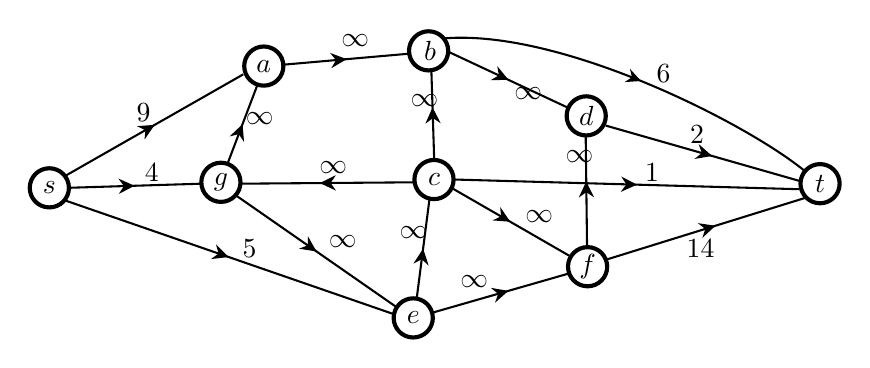
\begin{tikzpicture}[x=0.5pt,y=0.5pt,yscale=-1,xscale=1]
%uncomment if require: \path (0,271); %set diagram left start at 0, and has height of 271

%Straight Lines [id:da5212458340621946] 
\draw [color={rgb, 255:red, 0; green, 0; blue, 0 }  ,draw opacity=1 ][line width=0.75]    (227.5,50) -- (319,42) ;
\draw [shift={(273.25,46)}, rotate = 175] [fill={rgb, 255:red, 0; green, 0; blue, 0 }  ,fill opacity=1 ][line width=0.08]  [draw opacity=0] (11.61,-5.58) -- (0,0) -- (11.61,5.58) -- (7.71,0) -- cycle    ;
%Straight Lines [id:da5107871061349898] 
\draw [color={rgb, 255:red, 0; green, 0; blue, 0 }  ,draw opacity=1 ][line width=0.75]    (433,81) -- (347.5,41) ;
\draw [shift={(390.25,61)}, rotate = 205.07] [fill={rgb, 255:red, 0; green, 0; blue, 0 }  ,fill opacity=1 ][line width=0.08]  [draw opacity=0] (11.61,-5.58) -- (0,0) -- (11.61,5.58) -- (7.71,0) -- cycle    ;
%Straight Lines [id:da33373699050559813] 
\draw [color={rgb, 255:red, 0; green, 0; blue, 0 }  ,draw opacity=1 ][line width=0.75]    (446,101) -- (447,182) ;
\draw [shift={(446.41,134.4)}, rotate = 89.29] [fill={rgb, 255:red, 0; green, 0; blue, 0 }  ,fill opacity=1 ][line width=0.08]  [draw opacity=0] (11.61,-5.58) -- (0,0) -- (11.61,5.58) -- (7.71,0) -- cycle    ;
%Straight Lines [id:da41415742704032066] 
\draw [color={rgb, 255:red, 0; green, 0; blue, 0 }  ,draw opacity=1 ][line width=0.75]    (336,229) -- (433.5,201) ;
\draw [shift={(390.13,213.45)}, rotate = 163.98] [fill={rgb, 255:red, 0; green, 0; blue, 0 }  ,fill opacity=1 ][line width=0.08]  [draw opacity=0] (11.61,-5.58) -- (0,0) -- (11.61,5.58) -- (7.71,0) -- cycle    ;
%Straight Lines [id:da5297018905877636] 
\draw [color={rgb, 255:red, 0; green, 0; blue, 0 }  ,draw opacity=1 ][line width=0.75]    (336.5,118) -- (334.5,55) ;
\draw [shift={(335.32,80.9)}, rotate = 88.18] [fill={rgb, 255:red, 0; green, 0; blue, 0 }  ,fill opacity=1 ][line width=0.08]  [draw opacity=0] (11.61,-5.58) -- (0,0) -- (11.61,5.58) -- (7.71,0) -- cycle    ;
%Straight Lines [id:da9441285731905983] 
\draw [color={rgb, 255:red, 0; green, 0; blue, 0 }  ,draw opacity=1 ][line width=0.75]    (209,64) -- (187,122) ;
\draw [shift={(198,93)}, rotate = 110.77] [fill={rgb, 255:red, 0; green, 0; blue, 0 }  ,fill opacity=1 ][line width=0.08]  [draw opacity=0] (11.61,-5.58) -- (0,0) -- (11.61,5.58) -- (7.71,0) -- cycle    ;
%Straight Lines [id:da3078405450216426] 
\draw [color={rgb, 255:red, 0; green, 0; blue, 0 }  ,draw opacity=1 ][line width=0.75]    (322,135) -- (197,136) ;
\draw [shift={(253.9,135.54)}, rotate = 359.54] [fill={rgb, 255:red, 0; green, 0; blue, 0 }  ,fill opacity=1 ][line width=0.08]  [draw opacity=0] (11.61,-5.58) -- (0,0) -- (11.61,5.58) -- (7.71,0) -- cycle    ;
%Straight Lines [id:da3541622648157198] 
\draw [color={rgb, 255:red, 0; green, 0; blue, 0 }  ,draw opacity=1 ][line width=0.75]    (309,225) -- (194,145) ;
\draw [shift={(251.5,185)}, rotate = 214.82] [fill={rgb, 255:red, 0; green, 0; blue, 0 }  ,fill opacity=1 ][line width=0.08]  [draw opacity=0] (11.61,-5.58) -- (0,0) -- (11.61,5.58) -- (7.71,0) -- cycle    ;
%Straight Lines [id:da720688848918495] 
\draw [color={rgb, 255:red, 0; green, 0; blue, 0 }  ,draw opacity=1 ][line width=0.75]    (434,188) -- (349,139) ;
\draw [shift={(391.5,163.5)}, rotate = 209.96] [fill={rgb, 255:red, 0; green, 0; blue, 0 }  ,fill opacity=1 ][line width=0.08]  [draw opacity=0] (11.61,-5.58) -- (0,0) -- (11.61,5.58) -- (7.71,0) -- cycle    ;
%Straight Lines [id:da4466024070919401] 
\draw [color={rgb, 255:red, 0; green, 0; blue, 0 }  ,draw opacity=1 ][line width=0.75]    (333,148) -- (324,218) ;
\draw [shift={(328.5,183)}, rotate = 97.33] [fill={rgb, 255:red, 0; green, 0; blue, 0 }  ,fill opacity=1 ][line width=0.08]  [draw opacity=0] (11.61,-5.58) -- (0,0) -- (11.61,5.58) -- (7.71,0) -- cycle    ;
%Straight Lines [id:da19156407920574714] 
\draw [color={rgb, 255:red, 0; green, 0; blue, 0 }  ,draw opacity=1 ][line width=0.75]    (198.5,57) -- (70.5,130) ;
\draw [shift={(134.5,93.5)}, rotate = 150.3] [fill={rgb, 255:red, 0; green, 0; blue, 0 }  ,fill opacity=1 ][line width=0.08]  [draw opacity=0] (11.61,-5.58) -- (0,0) -- (11.61,5.58) -- (7.71,0) -- cycle    ;
%Straight Lines [id:da6856541088604527] 
\draw [color={rgb, 255:red, 0; green, 0; blue, 0 }  ,draw opacity=1 ][line width=0.75]    (168.5,136) -- (71.5,139) ;
\draw [shift={(120,137.5)}, rotate = 178.23] [fill={rgb, 255:red, 0; green, 0; blue, 0 }  ,fill opacity=1 ][line width=0.08]  [draw opacity=0] (11.61,-5.58) -- (0,0) -- (11.61,5.58) -- (7.71,0) -- cycle    ;
%Straight Lines [id:da6199102597257959] 
\draw [color={rgb, 255:red, 0; green, 0; blue, 0 }  ,draw opacity=1 ][line width=0.75]    (306.5,230) -- (69.5,148) ;
\draw [shift={(188,189)}, rotate = 199.09] [fill={rgb, 255:red, 0; green, 0; blue, 0 }  ,fill opacity=1 ][line width=0.08]  [draw opacity=0] (11.61,-5.58) -- (0,0) -- (11.61,5.58) -- (7.71,0) -- cycle    ;
%Straight Lines [id:da9810487383568949] 
\draw [color={rgb, 255:red, 0; green, 0; blue, 0 }  ,draw opacity=1 ][line width=0.75]    (600.5,134) -- (460.5,94) ;
\draw [shift={(537.33,115.95)}, rotate = 195.95] [fill={rgb, 255:red, 0; green, 0; blue, 0 }  ,fill opacity=1 ][line width=0.08]  [draw opacity=0] (11.61,-5.58) -- (0,0) -- (11.61,5.58) -- (7.71,0) -- cycle    ;
%Curve Lines [id:da06719487778357702] 
\draw    (343.5,31) .. controls (428.5,24) and (563.5,93) .. (604.5,127) ;
\draw [shift={(486.03,61.78)}, rotate = 201.88] [fill={rgb, 255:red, 0; green, 0; blue, 0 }  ][line width=0.08]  [draw opacity=0] (10.72,-5.15) -- (0,0) -- (10.72,5.15) -- (7.12,0) -- cycle    ;
%Straight Lines [id:da5887320294982179] 
\draw [color={rgb, 255:red, 0; green, 0; blue, 0 }  ,draw opacity=1 ][line width=0.75]    (605.5,146) -- (460.5,191) ;
\draw [shift={(539.78,166.4)}, rotate = 162.76] [fill={rgb, 255:red, 0; green, 0; blue, 0 }  ,fill opacity=1 ][line width=0.08]  [draw opacity=0] (11.61,-5.58) -- (0,0) -- (11.61,5.58) -- (7.71,0) -- cycle    ;
%Straight Lines [id:da573517504295797] 
\draw [color={rgb, 255:red, 0; green, 0; blue, 0 }  ,draw opacity=1 ][line width=0.75]    (600.5,140) -- (351.5,133) ;
\draw [shift={(483.1,136.7)}, rotate = 181.61] [fill={rgb, 255:red, 0; green, 0; blue, 0 }  ,fill opacity=1 ][line width=0.08]  [draw opacity=0] (11.61,-5.58) -- (0,0) -- (11.61,5.58) -- (7.71,0) -- cycle    ;

% Text Node
\draw (119.24,76.06) node [anchor=north west][inner sep=0.75pt]   [align=left] {$\displaystyle 9$};
% Text Node
\draw  [line width=1.5]   (182.38, 135) circle [x radius= 14.15, y radius= 14.15]   ;
\draw (182.38,135) node   [align=left] {$\displaystyle g$};
% Text Node
\draw  [line width=1.5]   (213.38, 51) circle [x radius= 14.15, y radius= 14.15]   ;
\draw (213.38,51) node   [align=left] {$\displaystyle a$};
% Text Node
\draw  [line width=1.5]   (332.48, 40) circle [x radius= 14.15, y radius= 14.15]   ;
\draw (326.98,40) node [anchor=west] [inner sep=0.75pt]   [align=left] {$\displaystyle b$};
% Text Node
\draw  [line width=1.5]   (336.38, 133) circle [x radius= 14.15, y radius= 14.15]   ;
\draw (336.38,133) node   [align=left] {$\displaystyle c$};
% Text Node
\draw  [line width=1.5]   (446.38, 87) circle [x radius= 14.15, y radius= 14.15]   ;
\draw (446.38,87) node   [align=left] {$\displaystyle d$};
% Text Node
\draw  [line width=1.5]   (321.38, 233) circle [x radius= 14.15, y radius= 14.15]   ;
\draw (321.38,233) node   [align=left] {$\displaystyle e$};
% Text Node
\draw  [line width=1.5]   (447.38, 196) circle [x radius= 14.15, y radius= 14.15]   ;
\draw (447.38,196) node   [align=left] {$\displaystyle f$};
% Text Node
\draw (125.24,119.06) node [anchor=north west][inner sep=0.75pt]   [align=left] {$\displaystyle 4$};
% Text Node
\draw (519.24,92.06) node [anchor=north west][inner sep=0.75pt]   [align=left] {$\displaystyle 2$};
% Text Node
\draw (195.75,174) node [anchor=north west][inner sep=0.75pt]   [align=left] {$\displaystyle 5$};
% Text Node
\draw (495,48) node [anchor=north west][inner sep=0.75pt]   [align=left] {$\displaystyle 6$};
% Text Node
\draw (516.75,174) node [anchor=north west][inner sep=0.75pt]   [align=left] {$\displaystyle 14$};
% Text Node
\draw (486.75,119) node [anchor=north west][inner sep=0.75pt]   [align=left] {$\displaystyle 1$};
% Text Node
\draw  [line width=1.5]   (58.38, 139) circle [x radius= 14.15, y radius= 14.15]   ;
\draw (58.38,139) node   [align=left] {$\displaystyle s$};
% Text Node
\draw  [line width=1.5]   (615.38, 136) circle [x radius= 14.15, y radius= 14.15]   ;
\draw (615.38,136) node   [align=left] {$\displaystyle t$};
% Text Node
\draw (267.24,26.06) node [anchor=north west][inner sep=0.75pt]   [align=left] {$\displaystyle \infty $};
% Text Node
\draw (198.24,82.06) node [anchor=north west][inner sep=0.75pt]   [align=left] {$\displaystyle \infty $};
% Text Node
\draw (251.24,118.06) node [anchor=north west][inner sep=0.75pt]   [align=left] {$\displaystyle \infty $};
% Text Node
\draw (258.24,171.06) node [anchor=north west][inner sep=0.75pt]   [align=left] {$\displaystyle \infty $};
% Text Node
\draw (309.24,165.06) node [anchor=north west][inner sep=0.75pt]   [align=left] {$\displaystyle \infty $};
% Text Node
\draw (353.24,200.06) node [anchor=north west][inner sep=0.75pt]   [align=left] {$\displaystyle \infty $};
% Text Node
\draw (400.24,153.06) node [anchor=north west][inner sep=0.75pt]   [align=left] {$\displaystyle \infty $};
% Text Node
\draw (429.24,110.06) node [anchor=north west][inner sep=0.75pt]   [align=left] {$\displaystyle \infty $};
% Text Node
\draw (317.24,69.06) node [anchor=north west][inner sep=0.75pt]   [align=left] {$\displaystyle \infty $};
% Text Node
\draw (392.25,64) node [anchor=north west][inner sep=0.75pt]   [align=left] {$\displaystyle \infty $};


\end{tikzpicture}

